\documentclass[]{article}
\usepackage{amsfonts}
\usepackage{pgfplots}
\usetikzlibrary{math}
\usepackage{amsmath}
\usepackage{lmodern}
\usepackage[T1]{fontenc}
\usepackage{setspace}
%\usepackage{fullpage}
%\pgfplotsset{compat=1.15}

\renewcommand{\div}{\mathrm {div}}
\DeclareMathOperator{\curl}{curl}
\DeclareMathOperator{\ran}{ran}

\definecolor{newcolor}{RGB}{.8,.349,.1}
\definecolor{lightgray}{RGB}{200,200,200}
%%%%%emph colors
\definecolor{emph1}{RGB}{0,102,153}
\definecolor{emph2}{RGB}{200,90,20}
\definecolor{emph3}{RGB}{100,30,153}
\definecolor{emph4}{RGB}{0,100,0}
\definecolor{emph5}{RGB}{0,100,200}
\definecolor{emph6}{RGB}{100,0,0}

%for image output uncomment the following two lines and the pgf plot paragraph and compile with --shell-escape
\usepgfplotslibrary{external}
\tikzexternalize[prefix=./]


\begin{document}


%%%%macros for drawing dofs
\newcommand{\trig}{%
  \draw[thick,gray](0,0)--++(4,0)--++(-4,4)--++(0,-4);
    \draw(0+2,0)--(0+4/3,0+4/3)--(0,0+2);
    \draw(0+2,0+2)--(0+4/3,0+4/3);
    }
\newcommand{\trigmethod}{%
  %\filldraw[fill=orange!30,thick,draw=gray](0,0)--++(4,0)--++(-4,4)--++(0,-4);
  \draw[thick](0,0)--++(4,0)--++(-4,4)--++(0,-4);
    %\filldraw[fill=orange!30](0+2,0)--(0+4/3,0+4/3)--(0,0+2);
    %\filldraw[fill=orange!30](0+2,0+2)--(0+4/3,0+4/3);
    \draw(0+2,0)--(0+4/3,0+4/3)--(0,0+2);
    \draw(0+2,0+2)--(0+4/3,0+4/3);
    \fill[fill=orange!30](0,0)--(0+2,0)--(0+4/3,0+4/3)--(0,0+2)--(0,0);
    }
\newcommand\dof[4][]{%
  \node[#1] at (2*#2-4/6*#2*#3,2*#3-4/6*#2*#3){};
  \node[] at (2*#2-4/6*#2*#3-0.1,2*#3-4/6*#2*#3-0.3){\small #4};
  %\node[#1] at (2*#3-4/6*#2*#3,4-2*#2+4/6*#2*#3-2*#3+4/6*#2*#3){};
  %\node[#1] at (4-2*#2+4/6*#2*#3-2*#3+4/6*#2*#3,2*#2-4/6*#2*#3){};
}
\newcommand\dofprimal[4][]{%
  \node[#1] at (2*#2-4/6*#2*#3,2*#3-4/6*#2*#3){};
  \node[] at (2*#2-4/6*#2*#3-0.1,2*#3-4/6*#2*#3-0.3){\small #4};
  \node[#1] at (2*#3-4/6*#2*#3,4-2*#2+4/6*#2*#3-2*#3+4/6*#2*#3){};
  \node[#1] at (4-2*#2+4/6*#2*#3-2*#3+4/6*#2*#3,2*#2-4/6*#2*#3){};
}
\newcommand\innerdofprimal[2]{
  \dofprimal[circle,thick,draw=blue]{#1}{#2}{}
}
\newcommand\innerdof[2]{
  \dof[circle,thick,draw=blue]{#1}{#2}{}
}
\newcommand\innervdof[2]{
  \dof[circle,thick,draw=teal]{#1}{#2}{}
}
\newcommand\graydof[2]{
  \dof[circle,thick,fill=gray]{#1}{#2}{}
}
\newcommand\graydofpimal[2]{
  \dofprimal[circle,thick,fill=gray]{#1}{#2}{}
}
\newcommand\facedof[2]{
  \dof[circle,fill=purple]{#1}{#2}{}
}
\newcommand\facedofprimal[2]{
  \dofprimal[circle,fill=purple]{#1}{#2}{}
}
\newcommand\facedoflabel[3]{
  \dof[circle,fill=purple]{#1}{#2}{#3}
}
\newcommand\edgedof[2]{
  \dof[circle,fill=blue]{#1}{#2}{}
}
\newcommand\edgedofprimal[2]{
  \dofprimal[circle,fill=blue]{#1}{#2}{}
}
\newcommand\edgedoflabel[3]{
  \dof[circle,fill=blue]{#1}{#2}{#3}
}
\newcommand\vertexdof[2]{
  \dof[circle,fill=teal]{#1}{#2}{}
}
\newcommand\vertexdofprimal[2]{
  \dofprimal[circle,fill=teal]{#1}{#2}{}
}
\newcommand\vertexdoflabel[3]{
  \dof[circle,fill=teal]{#1}{#2}{#3}
}
\newcommand\arrowdof[6][]{
  \begin{scope}[]
    \draw[#1,very thick,-latex] (2*#2-4/6*#2*#3,2*#3-4/6*#2*#3)--node {#6}                 (2*#4-4/6*#4*#5,2*#5-4/6*#4*#5);
  %\draw[#1,very thick,-latex] (2*#3-4/6*#2*#3,4-2*#2+4/6*#2*#3-2*#3+4/6*#2*#3)--(2*#5-4/6*#4*#5,4-2*#4+4/6*#4*#5-2*#5+4/6*#4*#5);
  %\draw[#1,very thick,-latex] (4-2*#2+4/6*#2*#3-2*#3+4/6*#2*#3,2*#2-4/6*#2*#3)--(4-2*#4+4/6*#4*#5-2*#5+4/6*#4*#5,2*#4-4/6*#4*#5);
  \end{scope}
}
\newcommand\arrowdofprimal[6][]{
  \begin{scope}[]
    \draw[#1,very thick,-latex] (2*#2-4/6*#2*#3,2*#3-4/6*#2*#3)--node {#6}                 (2*#4-4/6*#4*#5,2*#5-4/6*#4*#5);
  \draw[#1,very thick,-latex] (2*#3-4/6*#2*#3,4-2*#2+4/6*#2*#3-2*#3+4/6*#2*#3)--(2*#5-4/6*#4*#5,4-2*#4+4/6*#4*#5-2*#5+4/6*#4*#5);
  \draw[#1,very thick,-latex] (4-2*#2+4/6*#2*#3-2*#3+4/6*#2*#3,2*#2-4/6*#2*#3)--(4-2*#4+4/6*#4*#5-2*#5+4/6*#4*#5,2*#4-4/6*#4*#5);
  \end{scope}
}
\newcommand\facearrowdof[4]{
  \arrowdof[purple]{#1}{#2}{#3}{#4}{}
}
\newcommand\edgearrowdof[4]{
  \arrowdof[blue]{#1}{#2}{#3}{#4}{}
}
\newcommand\innerarrowdof[4]{
  \arrowdof[blue,dotted]{#1}{#2}{#3}{#4}{}
}

\newcommand\facearrowdofprimal[4]{
  \arrowdofprimal[purple]{#1}{#2}{#3}{#4}{}
}
\newcommand\edgearrowdofprimal[4]{
  \arrowdofprimal[blue]{#1}{#2}{#3}{#4}{}
}
\newcommand\innerarrowdofprimal[4]{
  \arrowdofprimal[blue,dotted]{#1}{#2}{#3}{#4}{}
}

\tikzsetnextfilename{ring_resonator_geo}
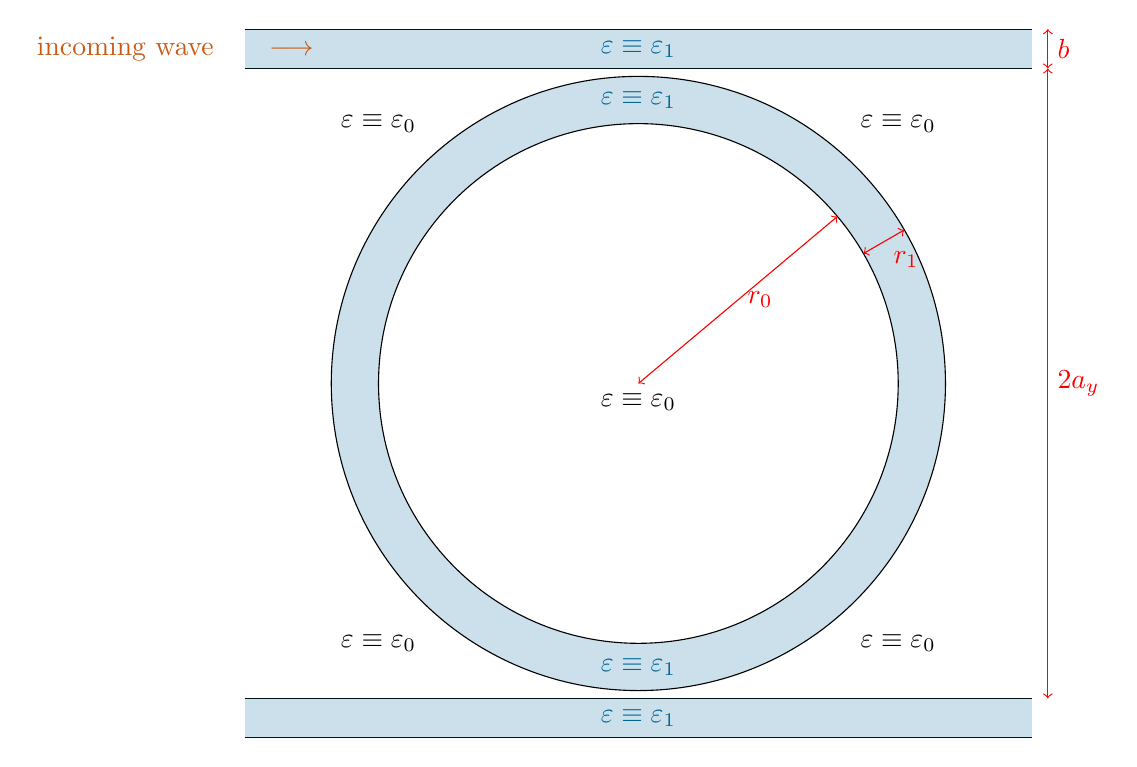
\begin{tikzpicture}
  \def\a{4};  
  \def\b{0.5};  
  \def\c{0.2};  
  \def\p{1};  
  \def\r{3.9};  
  \def\rr{3.3};  
  %\draw[] (-\a,-\a-\b-\c)--++(2*\a,0)--++(0,2*\a+2*\b+2*\c)--++(-2*\a,0)--++(0,-2*\a-2*\b-2*\c);
  %\draw[] (-\a-\p,\a)--++(2*\a+2*\p,0);
  \draw[] (-\a-\p,\a)--++(2*\a+2*\p,0);
  \draw[] (-\a-\p,\a+\b)--++(2*\a+2*\p,0);
  %\draw[] (-\a-\p,\a+\b+\c)--++(2*\a+2*\p,0);
  \draw[] (-\a-\p,-\a)--++(2*\a+2*\p,0);
  \draw[] (-\a-\p,-\a-\b)--++(2*\a+2*\p,0);
  %\draw[] (-\a-\p,-\a-\b-\c)--++(2*\a+2*\p,0);
  %\draw[] (-\a,-\a-\b-\c-\p)--++(-\p,\p)--++(0,2*\a+2*\b+2*\c)--++(\p,\p);
  %\draw[] (\a,-\a-\b-\c-\p)--++(\p,\p)--++(0,2*\a+2*\b+2*\c)--++(-\p,\p);
  %\fill[opacity=0.2] (\a,-\a-\b-\c-\p)--++(\p,\p)--++(0,2*\a+2*\b+2*\c)--++(-\p,\p);
  %\fill[opacity=0.2] (-\a,-\a-\b-\c-\p)--++(-\p,\p)--++(0,2*\a+2*\b+2*\c)--++(\p,\p);
  %\fill[opacity=0.2] (-\a,-\a-\b-\c-\p)--++(0,\p)--++(2*\a,0)--++(0,-\p);
  %\fill[opacity=0.2] (-\a,\a+\b+\c)--++(0,\p)--++(2*\a,0)--++(0,-\p);
  \fill[emph1,opacity=0.2] (-\a-\p,\a)--++(0,\b)--++(2*\a+2*\p,0)--++(0,-\b);
  \fill[emph1,opacity=0.2] (-\a-\p,-\a-\b)--++(0,\b)--++(2*\a+2*\p,0)--++(0,-\b);
  \fill[emph1,opacity=0.2,even odd rule] (0,0) circle (\r) (0,0) circle (\rr);
  \draw (0,0) circle (\r);
  \draw (0,0) circle (\rr);
  \node[left,emph2] at (-\a,\a+0.5*\b){incoming wave\qquad $\longrightarrow$};
  \node[emph1] at (0,\a+\b/2) {$\varepsilon\equiv\varepsilon_1$};
  \node[emph1] at (0,-\a-\b/2) {$\varepsilon\equiv\varepsilon_1$};
  \node[emph1] at (0,\r/2+\rr/2) {$\varepsilon\equiv\varepsilon_1$};
  \node[emph1] at (0,-\r/2-\rr/2) {$\varepsilon\equiv\varepsilon_1$};
  \node[below] at (0,0) {$\varepsilon\equiv\varepsilon_0$};
  \node[] at (\rr,\rr) {$\varepsilon\equiv\varepsilon_0$};
  \node[] at (-\rr,-\rr) {$\varepsilon\equiv\varepsilon_0$};
  \node[] at (-\rr,\rr) {$\varepsilon\equiv\varepsilon_0$};
  \node[] at (\rr,-\rr) {$\varepsilon\equiv\varepsilon_0$};
  %measurements
  %\draw[<->, red] (\a+\p+\c,\a+\b+\c+\p)--node[right]{$p$}++(0,-\p);
  %\draw[<->, red] (\a+\p+\c,\a+\b+\c)--node[right]{$c$}++(0,-\c);
  \draw[<->, red] (\a+\p+\c,\a+\b)--node[right]{$b$}++(0,-\b);
  \draw[<->, red] (\a+\p+\c,\a)--node[right]{$2a_y$}++(0,-\a-\a);
  %\draw[<->, red] (-\a,\a+\b+\c+\p+\c)--node[above]{$2a_x$}++(\a+\a,0);
  \draw[<->, red] (0,0)--node[right]{$r_0$}++(40:\rr);
  \draw[<->, red] (30:\rr)--node[below right]{$r_1$}(30:\r);
\end{tikzpicture}

\tikzsetnextfilename{ring_resonator_geo_pml}
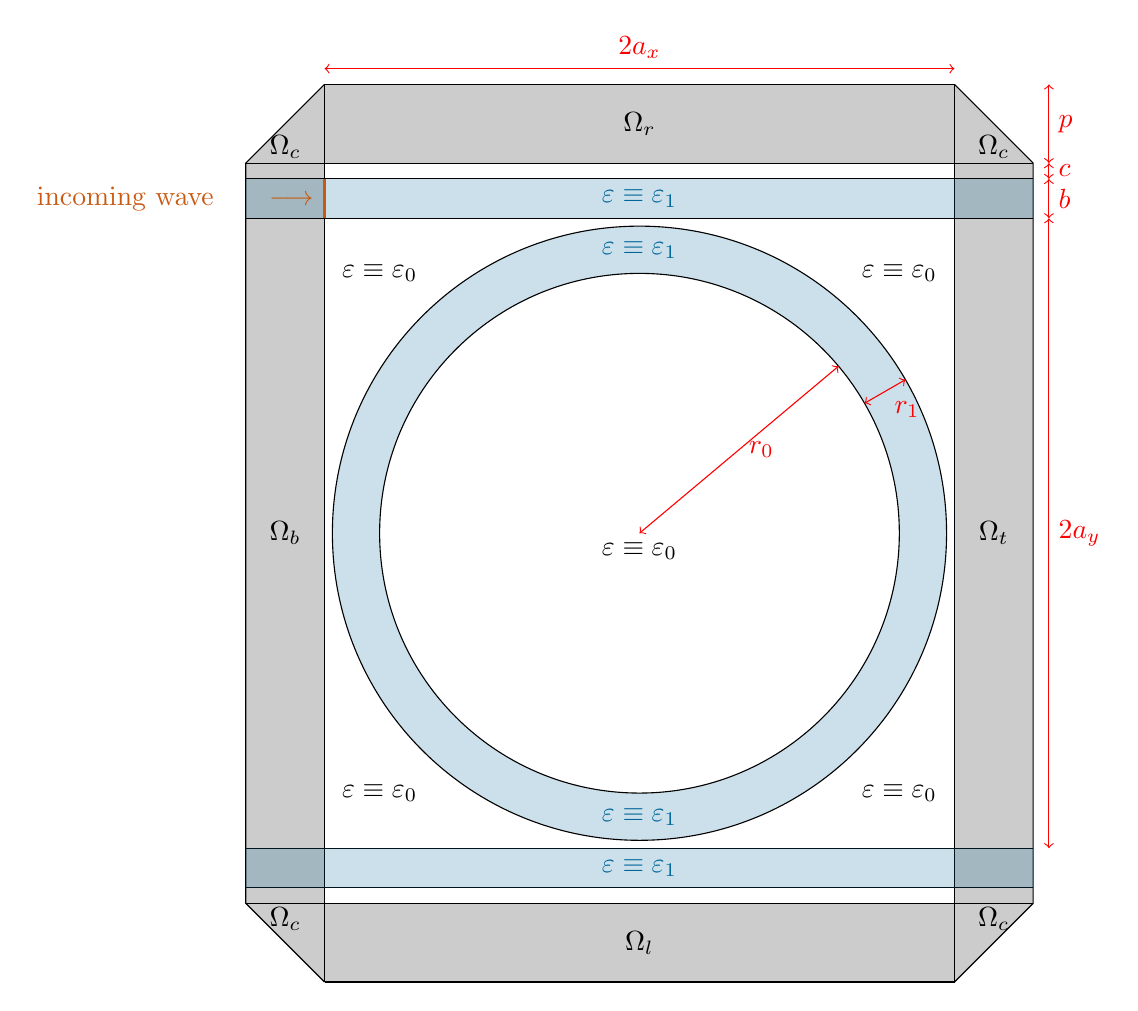
\begin{tikzpicture}
  \def\a{4};  
  \def\b{0.5};  
  \def\c{0.2};  
  \def\p{1};  
  \def\r{3.9};  
  \def\rr{3.3};  
  \draw[] (-\a,-\a-\b-\c-\p)--++(2*\a,0)--++(0,2*\a+2*\b+2*\c+2*\p)--++(-2*\a,0)--++(0,-2*\a-2*\b-2*\c-2*\p);
  \draw[] (-\a-\p,\a)--++(2*\a+2*\p,0);
  \draw[] (-\a-\p,\a)--++(2*\a+2*\p,0);
  \draw[] (-\a-\p,\a+\b)--++(2*\a+2*\p,0);
  \draw[] (-\a-\p,\a+\b+\c)--++(2*\a+2*\p,0);
  \draw[] (-\a-\p,-\a)--++(2*\a+2*\p,0);
  \draw[] (-\a-\p,-\a-\b)--++(2*\a+2*\p,0);
  \draw[] (-\a-\p,-\a-\b-\c)--++(2*\a+2*\p,0);
  \draw[] (-\a,-\a-\b-\c-\p)--++(-\p,\p)--++(0,2*\a+2*\b+2*\c)--++(\p,\p);
  \draw[] (\a,-\a-\b-\c-\p)--++(\p,\p)--++(0,2*\a+2*\b+2*\c)--++(-\p,\p);
  \fill[opacity=0.2] (\a,-\a-\b-\c-\p)--++(\p,\p)--++(0,2*\a+2*\b+2*\c)--++(-\p,\p);
  \fill[opacity=0.2] (-\a,-\a-\b-\c-\p)--++(-\p,\p)--++(0,2*\a+2*\b+2*\c)--++(\p,\p);
  \fill[opacity=0.2] (-\a,-\a-\b-\c-\p)--++(0,\p)--++(2*\a,0)--++(0,-\p);
  \fill[opacity=0.2] (-\a,\a+\b+\c)--++(0,\p)--++(2*\a,0)--++(0,-\p);
  \fill[emph1,opacity=0.2] (-\a-\p,\a)--++(0,\b)--++(2*\a+2*\p,0)--++(0,-\b);
  \fill[emph1,opacity=0.2] (-\a-\p,-\a-\b)--++(0,\b)--++(2*\a+2*\p,0)--++(0,-\b);
  \fill[emph1,opacity=0.2,even odd rule] (0,0) circle (\r) (0,0) circle (\rr);
  \draw (0,0) circle (\r);
  \draw (0,0) circle (\rr);
  \draw[very thick, emph2] (-\a,\a)--node[left]{incoming wave\qquad $\longrightarrow$}++(0,\b);
  \node at (0,\a+\b+\c+\p/2) {$\Omega_r$};
  \node at (0,-\a-\b-\c-\p/2) {$\Omega_l$};
  \node at (\a+\b+\c-\p/5,0) {$\Omega_t$};
  \node at (-\a-\b-\c+\p/5,0) {$\Omega_b$};
  \node at (-\a-\b-\c+\p/5,-\a-\b-\c-\p/5) {$\Omega_c$};
  \node at (+\a+\b+\c-\p/5,-\a-\b-\c-\p/5) {$\Omega_c$};
  \node at (-\a-\b-\c+\p/5,\a+\b+\c+\p/5) {$\Omega_c$};
  \node at (+\a+\b+\c-\p/5,\a+\b+\c+\p/5) {$\Omega_c$};
  \node[emph1] at (0,\a+\b/2) {$\varepsilon\equiv\varepsilon_1$};
  \node[emph1] at (0,-\a-\b/2) {$\varepsilon\equiv\varepsilon_1$};
  \node[emph1] at (0,\r/2+\rr/2) {$\varepsilon\equiv\varepsilon_1$};
  \node[emph1] at (0,-\r/2-\rr/2) {$\varepsilon\equiv\varepsilon_1$};
  \node[below] at (0,0) {$\varepsilon\equiv\varepsilon_0$};
  \node[] at (\rr,\rr) {$\varepsilon\equiv\varepsilon_0$};
  \node[] at (-\rr,-\rr) {$\varepsilon\equiv\varepsilon_0$};
  \node[] at (-\rr,\rr) {$\varepsilon\equiv\varepsilon_0$};
  \node[] at (\rr,-\rr) {$\varepsilon\equiv\varepsilon_0$};
  %measurements
  \draw[<->, red] (\a+\p+\c,\a+\b+\c+\p)--node[right]{$p$}++(0,-\p);
  \draw[<->, red] (\a+\p+\c,\a+\b+\c)--node[right]{$c$}++(0,-\c);
  \draw[<->, red] (\a+\p+\c,\a+\b)--node[right]{$b$}++(0,-\b);
  \draw[<->, red] (\a+\p+\c,\a)--node[right]{$2a_y$}++(0,-\a-\a);
  \draw[<->, red] (-\a,\a+\b+\c+\p+\c)--node[above]{$2a_x$}++(\a+\a,0);
  \draw[<->, red] (0,0)--node[right]{$r_0$}++(40:\rr);
  \draw[<->, red] (30:\rr)--node[below right]{$r_1$}(30:\r);
\end{tikzpicture}



\tikzsetnextfilename{dual_mesh_left}
        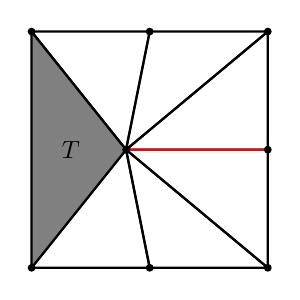
\begin{tikzpicture}[thick,scale=3.0, every node/.style={scale=3.0}]
        \coordinate (p1) at (0.0,0.0);
        \coordinate (p2) at (0.5,0.0);
        \coordinate (p3) at (1.0,0.0);
        \coordinate (p4) at (0.4,0.5);
        \coordinate (p5) at (1.0,0.5);
        \coordinate (p6) at (0.0,1.0);
        \coordinate (p7) at (0.5,1.0);
        \coordinate (p8) at (1.0,1.0);  
        \draw (p1) -- (p2) -- (p4) -- (p1);
        \draw[fill=gray] (p1) -- (p4) -- (p6) -- (p1);
        \draw (p4) -- (p6) -- (p7) -- (p4);
        \draw (p4) -- (p2) -- (p3) -- (p4);
        \draw (p4) -- (p3) -- (p5) -- (p4);
        \draw (p4) -- (p7) -- (p8) -- (p4);
        \draw (p4) -- (p8) -- (p5) -- (p4);
        \draw[color=red] (p4) -- (p5);
        % \node[scale=0.3] at (0.4+0.07,1/2+0.1) {$\mathbf{v}$};
        % \node[scale=0.3,color=red,thick] at (3/4,1/2+0.05) {$E$};
        \node[scale=0.3] at (1/6,1/2) {$T$};
        \node[circle,fill,scale=0.1] at (p1) {};
        \node[circle,fill,scale=0.1] at (p2) {};
        \node[circle,fill,scale=0.1] at (p3) {};
        \node[circle,fill,scale=0.1] at (p4) {};
        \node[circle,fill,scale=0.1] at (p5) {};
        \node[circle,fill,scale=0.1] at (p6) {};
        \node[circle,fill,scale=0.1] at (p7) {};
        \node[circle,fill,scale=0.1] at (p8) {};  
        \end{tikzpicture}
\tikzsetnextfilename{dual_mesh_center}

        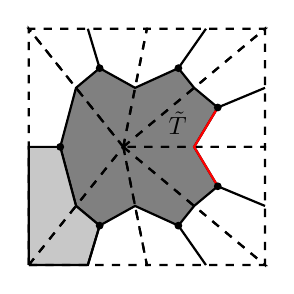
\begin{tikzpicture}[thick,scale=3.0, every node/.style={scale=3.0}]

          \coordinate (p1) at (0.0,0.0);
          \coordinate (p2) at (0.5,0.0);
          \coordinate (p3) at (1.0,0.0);
          \coordinate (p4) at (0.4,0.5);
          \coordinate (p5) at (1.0,0.5);
          \coordinate (p6) at (0.0,1.0);
          \coordinate (p7) at (0.5,1.0);
          \coordinate (p8) at (1.0,1.0);   
          \coordinate (p9) at (0.3000,0.1667);
          \coordinate (p10) at (0.1333,0.5000);
          \coordinate (p11) at (0.3000,0.8333);
          \coordinate (p12) at (0.6333,0.1667);
          \coordinate (p13) at (0.8000,0.3333);
          \coordinate (p14) at (0.8000,0.6667);
          \coordinate (p15) at (0.6333,0.8333);
          \coordinate (p16) at (0.2500,0);
          \coordinate (p17) at (0.2000,0.2500);
          \coordinate (p18) at (0.0,0.5000);
          \coordinate (p19) at (0.7500,0);
          \coordinate (p20) at (0.4500,0.2500);
          \coordinate (p21) at (0.7000,0.2500);
          \coordinate (p22) at (1.0000,0.2500);
          \coordinate (p23) at (0.7000,0.5000);
          \coordinate (p24) at (0.2000,0.7500);
          \coordinate (p25) at (0.4500,0.7500);
          \coordinate (p26) at (0.7000,0.7500);
          \coordinate (p27) at (1.0000,0.7500);
          \coordinate (p28) at (0.2500,1.0000);
          \coordinate (p29) at (0.7500,1.0000);
          \draw[fill=gray] (p13) -- (p23) -- (p14) -- (p26) -- (p15) -- (p25) -- (p11) -- (p24) --
                           (p10) -- (p17) -- (p9) -- (p20) -- (p12) -- (p21) -- (p13);
          \draw[fill=lightgray] (p1) -- (p16) -- (p9) -- (p17) -- (p10) -- (p18) -- (p1);
          \draw[dashed] (p1) -- (p2) -- (p4) -- (p1);
          \draw[dashed] (p1) -- (p4) -- (p6) -- (p1);
          \draw[dashed] (p4) -- (p6) -- (p7) -- (p4);
          \draw[dashed] (p4) -- (p2) -- (p3) -- (p4);
          \draw[dashed] (p4) -- (p3) -- (p5) -- (p4);
          \draw[dashed] (p4) -- (p7) -- (p8) -- (p4);
          \draw[dashed] (p4) -- (p8) -- (p5) -- (p4);
        \draw[color=black] (p16) -- (p9);
        \draw[color=black] (p19) -- (p12);
        \draw[color=black] (p22) -- (p13);
        \draw[color=black] (p27) -- (p14);
        \draw[color=black] (p29) -- (p15);
        \draw[color=black] (p28) -- (p11);
        \draw[color=black] (p18) -- (p10);
        \draw[color=red] (p13) -- (p23) -- (p14);
        \node[circle,fill,scale=0.1] at (p9) {};
        \node[circle,fill,scale=0.1] at (p10) {};
        \node[circle,fill,scale=0.1] at (p11) {};
        \node[circle,fill,scale=0.1] at (p12) {};
        \node[circle,fill,scale=0.1] at (p13) {};
        \node[circle,fill,scale=0.1] at (p14) {};
        \node[circle,fill,scale=0.1] at (p15) {}; 
        \node[scale=0.3] at (1/2+0.13,1/2+0.1) {$\tilde{T}$};
        % \node[scale=0.3,thick,color=red] at (5/6,1/2+0.07) {$\tilde{E}$};
        % \node[scale=0.3] at (1/9,3/7) {$\tilde{\mathbf{v}}$};
        \end{tikzpicture}
\tikzsetnextfilename{dual_mesh_right}
        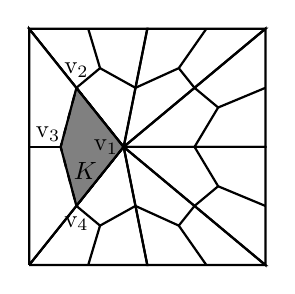
\begin{tikzpicture}[thick,scale=3.0, every node/.style={scale=3.0}]
          \coordinate (p1) at (0.0,0.0);
          \coordinate (p2) at (0.5,0.0);
          \coordinate (p3) at (1.0,0.0);
          \coordinate (p4) at (0.4,0.5);
          \coordinate (p5) at (1.0,0.5);
          \coordinate (p6) at (0.0,1.0);
          \coordinate (p7) at (0.5,1.0);
          \coordinate (p8) at (1.0,1.0);   
          \coordinate (p9) at (0.3000,0.1667);
          \coordinate (p10) at (0.1333,0.5000);
          \coordinate (p11) at (0.3000,0.8333);
          \coordinate (p12) at (0.6333,0.1667);
          \coordinate (p13) at (0.8000,0.3333);
          \coordinate (p14) at (0.8000,0.6667);
          \coordinate (p15) at (0.6333,0.8333);
          \coordinate (p16) at (0.2500,0);
          \coordinate (p17) at (0.2000,0.2500);
          \coordinate (p18) at (0,0.5000);
          \coordinate (p19) at (0.7500,0);
          \coordinate (p20) at (0.4500,0.2500);
          \coordinate (p21) at (0.7000,0.2500);
          \coordinate (p22) at (1.0000,0.2500);
          \coordinate (p23) at (0.7000,0.5000);
          \coordinate (p24) at (0.2000,0.7500);
          \coordinate (p25) at (0.4500,0.7500);
          \coordinate (p26) at (0.7000,0.7500);
          \coordinate (p27) at (1.0000,0.7500);
          \coordinate (p28) at (0.2500,1.0000);
          \coordinate (p29) at (0.7500,1.0000);
          \draw[dashed,fill=gray] (p4) -- (p24) -- (p10) --
                                  (p17) -- (p4);
          \draw            (p13) -- (p23) -- (p14) -- (p26) -- (p15) -- 
                           (p25) -- (p11) -- (p24) -- (p10) -- (p17) -- 
                           (p9) -- (p20) -- (p12) -- (p21) -- (p13);
          \draw (p1) -- (p2) -- (p4) -- (p1);
          \draw (p1) -- (p4) -- (p6) -- (p1);
          \draw (p4) -- (p6) -- (p7) -- (p4);
          \draw (p4) -- (p2) -- (p3) -- (p4);
          \draw (p4) -- (p3) -- (p5) -- (p4);
          \draw (p4) -- (p7) -- (p8) -- (p4);
          \draw (p4) -- (p8) -- (p5) -- (p4);
        \draw[color=black] (p16) -- (p9);
        \draw[color=black] (p19) -- (p12);
        \draw[color=black] (p22) -- (p13);
        \draw[color=black] (p27) -- (p14);
        \draw[color=black] (p29) -- (p15);
        \draw[color=black] (p28) -- (p11);
        \draw[color=black] (p18) -- (p10);
        \node[scale=0.3,left of=p4, node distance=2.5mm] (v1)  {$\mathrm v_1$};
        \node[scale=0.3,above of=p24, node distance=2.5mm] (v2) {$\mathrm v_2$};
        \node[scale=0.3,above left of=p10, node distance=2.5mm] (v3) {$\mathrm v_3$};
        \node[scale=0.3,below of=p17, node distance=2.5mm] (v4) {$\mathrm v_4$};
        % \draw[color=red] (p24) -- (p10) -- (p17);
        % \draw[color=green] (p24) -- (p4) -- (p17);
        \node[scale=0.3,below] at (0.95*1/4,0.95*1/2) {$K$};
        % \node[scale=0.3,thick,color=red] at (1/8,1/3) {$\tilde{e}$};
        % \node[scale=0.3,thick,color=green] at (1/3,2/3) {${e}$};
        \end{tikzpicture}

\end{document}:
